\chapter{ميكانيكا الكم للكيميائيين: الأنظمة النموذجية}\label{ch:b3:quantum-model-systems}

ثلاث قوارير صغيرة على طاولة المختبر، في كل منها محلول صبغة سيانينية
في الإيثانول: الأولى أرجوانية، والثانية زرقاء، والثالثة زرقاء مخضرّة
داكنة تمتص في الأحمر البعيد. الجزيئات الثلاثة مبنية على نمط واحد ---
حلقتان متطابقتان تحويان النيتروجين تصل بينهما سلسلة من ذرات الكربون ---
ولا تختلف إلا في طول هذه السلسلة، بذرتي كربون في كل مرة. فإذا طالت
السلسلة انزاح اللون نحو الأحمر. وقد فسّر كيميائي سنة 1949 هذه السلسلة
بواحدة من أبسط مسائل ميكانيكا الكم: إلكترون حر الحركة على خط طوله ثابت،
أي «\omterm{def:b3:quantum-model-systems:box}{جسيم في صندوق}». يضع هذا الفصل الأدوات التي يقوم عليها هذا التفسير
--- المؤثرات والقيم الذاتية \omterm{thm:b3:quantum-model-systems:schrodinger}{ومعادلة شرودنغر} --- ويحل الأنظمة النموذجية
التي تستعملها الكيمياء كل يوم: الصندوق، \omterm{def:b3:quantum-model-systems:oscillator}{والهزاز التوافقي} لرابطة تهتز،
\omterm{def:b3:quantum-model-systems:rotor}{والدوّار الصلب} لجزيء يدور، وذرة الهيدروجين، والحاجز الذي يستطيع جسيم
خفيف أن يعبره دون أن يملك الطاقة اللازمة لتسلّقه.

\begin{recall}
بيّن مجلد السنة الأولى أن طاقة الذرة مكمّاة (مستويات الطاقة، والحالة
الأساسية والحالات المثارة، وخطوط الهيدروجين) وأن الفوتون يحمل
$E = h\nu = hc/\lambda$. ووصف مجلد السنة الثانية الإلكترون بدالة موجية
$\psi$ مربعها كثافة احتمال، وفصل مدارات الهيدروجين إلى جزء شعاعي وجزء
زاوي، وعدّ عقدها؛ وقد أخذ الدوال الموجية للهيدروجين معطاة. وهي تُستنتج
هنا، في القسم 5. ومن الفيزياء: كمية الحركة $p = mv$ وطول موجة دي بروي
$\lambda = h/p$.
\end{recall}

\begin{omfigure}
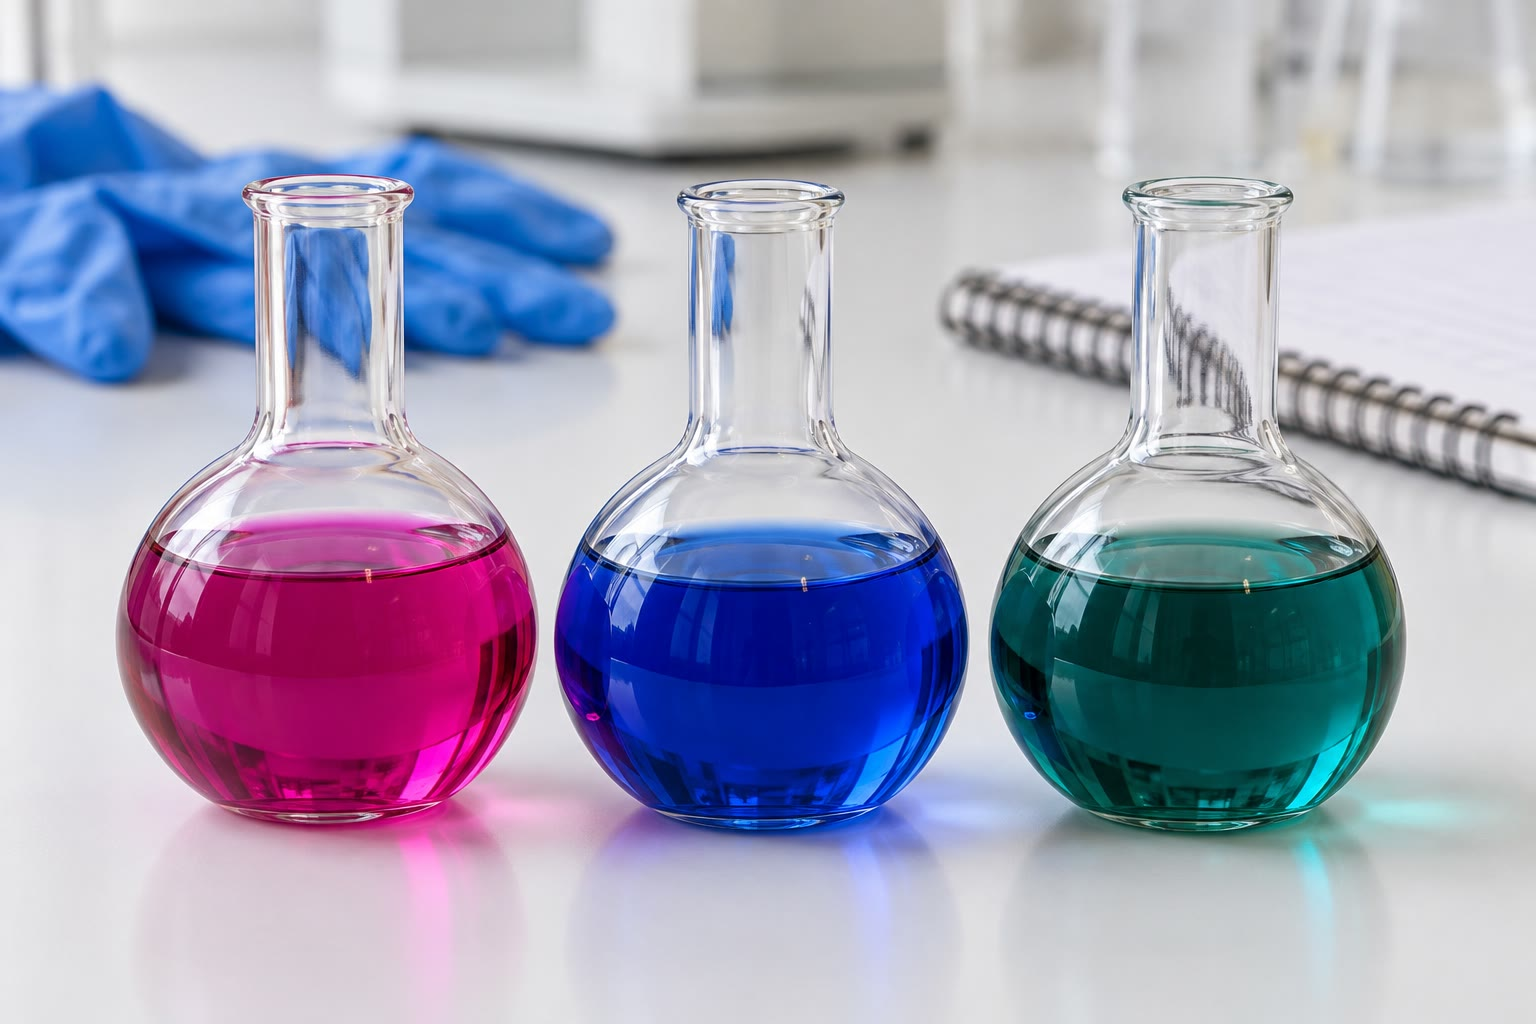
\includegraphics[width=0.62\linewidth]{images/book4/ai/b3-01-dyes.jpg}

{\small محاليل ثلاث صبغات سيانينية من عائلة واحدة. كل زوج من ذرات الكربون
يُضاف إلى السلسلة يزيح الامتصاص نحو الأحمر.}
\end{omfigure}

\section{المؤثرات والقيم الذاتية ومعادلة شرودنغر}

تمنح الميكانيكا الكلاسيكية الجسيم موضعًا وكمية حركة في كل لحظة. أما
ميكانيكا الكم فتمنحه حالة، هي الدالة الموجية $\psi$، وتستبدل بكل مقدار
قابل للقياس عمليةً تُجرى على $\psi$.

\begin{definition}[المؤثر، الدالة الذاتية، القيمة الذاتية]\label{def:b3:quantum-model-systems:operator}
\emph{المؤثر}\index{مؤثر} $\hat A$ قاعدة تحوّل دالةً إلى دالة أخرى:
$\hat A f = g$. ويكون خطيًا إذا تحقق $\hat A(\lambda f +
\mu g) = \lambda\hat Af + \mu\hat Ag$. والدالة غير المعدومة $f$ التي تحقق
$\hat Af = a f$ من أجل عدد $a$ هي \emph{دالة ذاتية}\index{دالة ذاتية}
للمؤثر $\hat A$، والعدد $a$ هو \emph{القيمة الذاتية}\index{قيمة ذاتية} الموافقة لها.
\end{definition}

\begin{example}[مؤثرا الموضع وكمية الحركة]\label{ex:b3:quantum-model-systems:xp}
في بُعد واحد يضرب \omterm{def:b3:quantum-model-systems:operator}{مؤثر} الموضع في $x$، أي $\hat x f = xf$،
ويشتق \omterm{def:b3:quantum-model-systems:operator}{مؤثر} كمية الحركة، $\hat p f = -\iu\hbar\,
\dd f/\dd x$، حيث $\hbar = h/2\pi$. والدالة $\eu^{\iu kx}$
\omterm{def:b3:quantum-model-systems:operator}{دالة ذاتية} \omterm{def:b3:quantum-model-systems:operator}{للمؤثر} $\hat p$ قيمتها الذاتية $\hbar k$: فالموجة التي طولها
$\lambda = 2\pi/k$ كمية حركتها $h/\lambda$، وهي علاقة دي بروي.
أما الدالة $\sin kx$ فليست \omterm{def:b3:quantum-model-systems:operator}{دالة ذاتية} \omterm{def:b3:quantum-model-systems:operator}{للمؤثر} $\hat p$ (مشتقتها
جيب تمام)، لكنها \omterm{def:b3:quantum-model-systems:operator}{دالة ذاتية} \omterm{def:b3:quantum-model-systems:operator}{للمؤثر} $\hat p^2 = -\hbar^2\,\dd^2/\dd x^2$، قيمتها
الذاتية $\hbar^2k^2$.
\end{example}

\begin{definition}[المؤثر الهرميتي، القيمة المتوقعة]\label{def:b3:quantum-model-systems:hermitian}
نكتب $\langle f|g\rangle = \int f^*g\,\dd\tau$ لدالتين تنعدمان
على حدود المنطقة. ويكون \omterm{def:b3:quantum-model-systems:operator}{المؤثر} \emph{هرميتيًا}\index{مؤثر هرميتي}
إذا تحقق $\langle f|\hat Ag\rangle = \langle \hat Af|g\rangle$ لكل دالتين من هذا النوع
$f$ و$g$. ومن أجل حالة منظَّمة $\psi$ ($\langle\psi|\psi\rangle = 1$)، تكون
\emph{القيمة المتوقعة}\index{قيمة متوقعة} \omterm{def:b3:quantum-model-systems:operator}{للمؤثر} $\hat A$ هي
$\langle A\rangle = \langle\psi|\hat A\psi\rangle$: متوسط قياسات
كثيرة تُجرى على أنظمة محضَّرة تحضيرًا متطابقًا.
\end{definition}

يمكن الآن أن تُصاغ قواعد العمل في كيمياء الكم --- أي مسلّماتها --- في
نَفَس واحد: يُمثَّل كل مقدار قابل للقياس \omterm{def:b3:quantum-model-systems:hermitian}{بمؤثر
هرميتي}؛ ويعطي القياس إحدى قيمه الذاتية؛ وإذا كانت
$\psi$ \omterm{def:b3:quantum-model-systems:operator}{دالة ذاتية} \omterm{def:b3:quantum-model-systems:operator}{للمؤثر} $\hat A$، أعطى كل قياس يُجرى عليها
القيمة نفسها، وهي قيمتها الذاتية.

\begin{theorem}[المؤثرات الهرميتية]\label{thm:b3:quantum-model-systems:hermitian-real}
القيم الذاتية \omterm{def:b3:quantum-model-systems:hermitian}{لمؤثر هرميتي} حقيقية. والدالتان الذاتيتان اللتان تختلف
قيمتاهما الذاتيتان متعامدتان: $\langle f_1|f_2\rangle = 0$.
\end{theorem}

\begin{proof}
ليكن $\hat Af = af$. عندئذ $\langle f|\hat Af\rangle = a\langle f|f\rangle$ 
و$\langle\hat Af|f\rangle = a^*\langle f|f\rangle$. \omterm{def:b3:quantum-model-systems:hermitian}{والمؤثر هرميتي}،
فهاتان الكميتان متساويتان، و$\langle f|f\rangle > 0$: إذن $a = a^*$. لنأخذ الآن $\hat Af_1
= a_1f_1$ و$\hat Af_2 = a_2f_2$ مع $a_1 \ne a_2$، وكلتاهما حقيقية. عندئذ
$\langle f_1|\hat Af_2\rangle = a_2\langle f_1|f_2\rangle$ و$\langle\hat Af_1|
f_2\rangle = a_1\langle f_1|f_2\rangle$؛ وتساويهما يعطي $(a_2 - a_1)
\langle f_1|f_2\rangle = 0$، ومنه $\langle f_1|f_2\rangle = 0$.
\end{proof}

القيمة المقيسة عدد حقيقي، ولهذا يجب أن تكون المقادير القابلة للقياس
هرميتية؛ والتعامد هو ما يجعل مدارات الذرة، أو مستويات الصندوق، مجموعة
نظيفة من الحالات المستقلة.

\begin{definition}[المبدِّل]\label{def:b3:quantum-model-systems:commutator}
\emph{المبدِّل}\index{مبدِّل} لمؤثرين هو $[\hat A,\hat B] =
\hat A\hat B - \hat B\hat A$. ويتبادل المؤثران إذا كان مبدِّلهما
معدومًا.
\end{definition}

\begin{example}[المبدِّل القانوني]\label{ex:b3:quantum-model-systems:canonical}
من أجل أي دالة $f$، $\hat x\hat pf = -\iu\hbar xf'$ و$\hat p\hat xf =
-\iu\hbar(f + xf')$. والفرق هو $[\hat x,\hat p]f = \iu\hbar f$، ومنه
$[\hat x,\hat p] = \iu\hbar$: الموضع وكمية الحركة لا يتبادلان. وعلى هذه
العلاقة الوحيدة يقوم مبدأ الارتياب، وفيما يلي، طيف \omterm{def:b3:quantum-model-systems:oscillator}{الهزاز التوافقي}
بأكمله.
\end{example}

\begin{proposition}[المؤثرات المتبادلة]\label{prop:b3:quantum-model-systems:commuting}
إذا تبادل $\hat A$ و$\hat B$ وكانت $f$ \omterm{def:b3:quantum-model-systems:operator}{دالة ذاتية} \omterm{def:b3:quantum-model-systems:operator}{للمؤثر} $\hat A$
\omterm{def:b3:quantum-model-systems:operator}{بقيمة ذاتية} غير منحلة $a$، فإن $f$ \omterm{def:b3:quantum-model-systems:operator}{دالة ذاتية} \omterm{def:b3:quantum-model-systems:operator}{للمؤثر}
$\hat B$ أيضًا.
\end{proposition}

\begin{proof}
$\hat A(\hat Bf) = \hat B\hat Af = a(\hat Bf)$: الدالة $\hat Bf$
\omterm{def:b3:quantum-model-systems:operator}{دالة ذاتية} \omterm{def:b3:quantum-model-systems:operator}{للمؤثر} $\hat A$ \omterm{def:b3:quantum-model-systems:operator}{بالقيمة الذاتية} نفسها $a$، أو معدومة. ولأن
\omterm{def:b3:quantum-model-systems:operator}{القيمة الذاتية} غير منحلة، فإن $\hat Bf$ مضاعف للدالة $f$، وليكن $bf$.
\end{proof}

\omterm{def:b3:quantum-model-systems:operator}{مؤثر} الطاقة هو \omterm{def:b3:quantum-model-systems:schrodinger}{مؤثر هاملتون}. فمن أجل جسيم كتلته $m$ في
كمون $V$، تصير الطاقة الكلاسيكية $p^2/2m + V$ مؤثرًا.

\begin{definition}[مؤثر هاملتون]\label{def:b3:quantum-model-systems:schrodinger}
\emph{مؤثر هاملتون}\index{مؤثر هاملتون} لجسيم
كتلته $m$ يتحرك في كمون $V(\mathbf r)$ هو
\[
\hat H = -\frac{\hbar^2}{2m}\nabla^2 + V(\mathbf r), \qquad \nabla^2 =
\frac{\partial^2}{\partial x^2} + \frac{\partial^2}{\partial y^2} +
\frac{\partial^2}{\partial z^2},
\]
ومن أجل عدة جسيمات، هو مجموع حدودها الحركية وجميع طاقاتها
الكامنة.
\end{definition}

\begin{theorem}[معادلة شرودنغر]\label{thm:b3:quantum-model-systems:schrodinger}
حالات النظام ذات الطاقة المحددة --- أي حالاته المستقرة --- هي
الدوال الذاتية \omterm{def:b3:quantum-model-systems:schrodinger}{لمؤثر هاملتون} الخاص به، وطاقاته المسموح بها هي
القيم الذاتية:
\[
\hat H\psi = E\psi,
\]
وهي \emph{معادلة شرودنغر}\index{معادلة شرودنغر} المستقلة عن الزمن.
والدالة $\psi$ المقبولة وحيدة القيمة ومتصلة
وقابلة للمكاملة تربيعيًا (يمكن تنظيمها).
\end{theorem}
\begin{proof}[مكانتها]
هذه مسلَّمة، يسوّغها ما يترتب عليها: فمستويات كل
نظام يُحل أدناه توافق المطيافية. أما المعادلة المتعلقة بالزمن،
التي هذه حالتها المستقرة، فمن شأن الفيزياء.
\end{proof}

الشروط الحدية هي التي تفرض التكميم: فللمعادلة التفاضلية
حلول من أجل كل $E$، لكن مجموعة منفصلة منها فقط تبقى منتهية
ومتصلة. فتصير الكيمياء عندئذ مسألة اختيار كمون، ثم الحل،
ثم قراءة القيم الذاتية.

\begin{method}[حل نموذج أحادي البعد]\label{met:b3:quantum-model-systems:one-dimensional}
\begin{enumerate}
  \item اكتب الكمون $V(x)$ \omterm{def:b3:quantum-model-systems:schrodinger}{ومؤثر هاملتون}؛ وقسّم الفضاء إلى
        مناطق يكون فيها $V$ بسيطًا.
  \item حُلّ $-\frac{\hbar^2}{2m}\psi'' + V\psi = E\psi$ في كل منطقة: دوال جيب
        وجيب تمام حيث $E > V$، ودوال أسية حقيقية حيث $E < V$.
  \item افرض الشروط: $\psi = 0$ حيث يكون $V$ لانهائيًا؛ و$\psi$
        و$\psi'$ متصلتان عند درجة منتهية؛ و$\psi \to 0$ عند اللانهاية.
  \item لا تتحقق الشروط إلا من أجل قيم معينة للطاقة $E$: وهي المستويات.
  \item نظّم كل \omterm{def:b3:quantum-model-systems:operator}{دالة ذاتية}؛ وعُدّ عقدها للتحقق (للمستوى
        رقم $n$ في مسألة أحادية البعد $n - 1$ عقدة).
\end{enumerate}
\end{method}

\section{الجسيم في صندوق}

\begin{definition}[الجسيم في صندوق، نموذج الإلكترون الحر]\label{def:b3:quantum-model-systems:box}
\emph{الجسيم في صندوق}\index{جسيم في صندوق} يتحرك بحرية ($V = 0$)
بين $x = 0$ و$x = L$ ولا يستطيع المغادرة ($V = \infty$ في الخارج). 
و\emph{نموذج الإلكترون الحر}\index{نموذج الإلكترون الحر} لجزيء
مترافق يعامل إلكترونات $\pi$ فيه جسيماتٍ مستقلة في صندوق
طوله طول السلسلة المترافقة.
\end{definition}

\begin{theorem}[مستويات الصندوق]\label{thm:b3:quantum-model-systems:box}
مستويات جسيم كتلته $m$ في صندوق طوله $L$ ودواله الذاتية المنظَّمة
هي
\[
E_n = \frac{n^2h^2}{8mL^2}, \qquad \psi_n(x) = \sqrt{\frac2L}\,\sin\frac{n\pi
x}{L}, \qquad n = 1, 2, 3, \dots
\]
\end{theorem}

\begin{proof}
في الداخل، $\psi'' = -k^2\psi$ حيث $k^2 = 2mE/\hbar^2$، ومنه $\psi = A\sin kx +
B\cos kx$. وفي الخارج $\psi = 0$، فيعطي الاتصال $\psi(0) = 0$، ومنه $B =
0$، و$\psi(L) = 0$، ومنه $\sin kL = 0$ مع $A \ne 0$: أي $kL = n\pi$، حيث $n$
عدد صحيح موجب ($n = 0$ يعطي $\psi = 0$؛ والقيم السالبة للعدد $n$ تكرر الدوال
نفسها). عندئذ $E = \hbar^2k^2/2m = n^2\pi^2\hbar^2/2mL^2 = n^2h^2/8mL^2$.
وأخيرًا يعطي $\int_0^L A^2\sin^2(n\pi x/L)\,\dd x = A^2L/2 = 1$ القيمة $A =
\sqrt{2/L}$.
\end{proof}

ثلاث سمات تنتقل إلى كل نظام مقيَّد: أدنى طاقة ليست
معدومة (لا يمكن للجسيم أن يسكن أبدًا)، وتتباعد المستويات كلما كبر $n$،
وتتقارب كلما كبر الصندوق ($E \propto 1/L^2$): فالصندوق
الكبير كلاسيكي تقريبًا.

\begin{omfigure}
\begin{tikzpicture}
\begin{axis}[width=0.5\linewidth, height=6.4cm, xmin=-0.08, xmax=1.08,
  ymin=0, ymax=18.4, axis lines=left, xtick={0,1}, xticklabels={$0$,$L$},
  ytick={1,4,9,16}, yticklabels={$E_1$,$4E_1$,$9E_1$,$16E_1$},
  tick label style={font=\small}, xlabel={$x$}, title={\small $\psi_n$}]
\foreach \n in {1,4,9,16}{\addplot[gray!50, dashed, domain=0:1] {\n};}
\addplot[omDef, thick] table[x=x, y=p1] {figdata/out/bachelor-3-particle-in-box.dat};
\addplot[omDef, thick] table[x=x, y=p2] {figdata/out/bachelor-3-particle-in-box.dat};
\addplot[omDef, thick] table[x=x, y=p3] {figdata/out/bachelor-3-particle-in-box.dat};
\addplot[omDef, thick] table[x=x, y=p4] {figdata/out/bachelor-3-particle-in-box.dat};
\draw[very thick] (axis cs:0,0) -- (axis cs:0,18.4) (axis cs:1,0) -- (axis cs:1,18.4);
\end{axis}
\end{tikzpicture}\hspace{0.5em}%
\begin{tikzpicture}
\begin{axis}[width=0.5\linewidth, height=6.4cm, xmin=-0.08, xmax=1.08,
  ymin=0, ymax=18.4, axis lines=left, xtick={0,1}, xticklabels={$0$,$L$},
  ytick={1,4,9,16}, yticklabels={$n=1$,$n=2$,$n=3$,$n=4$},
  tick label style={font=\small}, xlabel={$x$}, title={\small $|\psi_n|^2$}]
\foreach \n in {1,4,9,16}{\addplot[gray!50, dashed, domain=0:1] {\n};}
\addplot[omThm, thick] table[x=x, y=d1] {figdata/out/bachelor-3-particle-in-box.dat};
\addplot[omThm, thick] table[x=x, y=d2] {figdata/out/bachelor-3-particle-in-box.dat};
\addplot[omThm, thick] table[x=x, y=d3] {figdata/out/bachelor-3-particle-in-box.dat};
\addplot[omThm, thick] table[x=x, y=d4] {figdata/out/bachelor-3-particle-in-box.dat};
\draw[very thick] (axis cs:0,0) -- (axis cs:0,18.4) (axis cs:1,0) -- (axis cs:1,18.4);
\end{axis}
\end{tikzpicture}

{\small المستويات الأربعة الأولى \omterm{def:b3:quantum-model-systems:box}{لجسيم في صندوق}، كل دالة مرسومة على
مستواها (متقطع). يسارًا: $\psi_n$، ولها $n - 1$ عقدة داخل الصندوق.
يمينًا: كثافة الاحتمال $|\psi_n|^2$.}
\end{omfigure}

\begin{proposition}[الصندوق المكعب]\label{prop:b3:quantum-model-systems:box-3d}
في صندوق مكعب ضلعه $L$، $\psi = \psi_{n_x}(x)\psi_{n_y}(y)\psi_{n_z}(z)$ 
و$E = (n_x^2 + n_y^2 + n_z^2)\,h^2/8mL^2$. والثلاثيات المختلفة التي لها مجموع
المربعات نفسه تعطي الطاقة نفسها.
\end{proposition}

\begin{proof}
بما أن $V = 0$ في الداخل، فإن $\hat H$ مجموع ثلاثة مؤثرات أحادية البعد،
واحد لكل إحداثي. وجداء ثلاث دوال ذاتية أحادية البعد
\omterm{def:b3:quantum-model-systems:operator}{دالة ذاتية} للمجموع، قيمتها الذاتية مجموع القيم الذاتية الثلاث؛ وهو
ينعدم على كل وجه، كما هو مطلوب.
\end{proof}

\begin{definition}[المستويات المنحلة]\label{def:b3:quantum-model-systems:degenerate}
الدوال الذاتية المستقلة خطيًا التي لها \omterm{def:b3:quantum-model-systems:operator}{القيمة الذاتية} نفسها
\emph{مستويات منحلة}\index{مستويات منحلة}؛ وعددها هو
\emph{درجة الانحلال}\index{درجة الانحلال} $g$ لتلك الطاقة.
\end{definition}

\begin{example}[الانحلال والتناظر]\label{ex:b3:quantum-model-systems:cube}
ينتج المستوى $n_x^2 + n_y^2 + n_z^2 = 6$ للمكعب عن $(2,1,1)$
و$(1,2,1)$ و$(1,1,2)$: أي $g = 3$. فإذا مُطّ الصندوق قليلًا على امتداد $z$
ابتعدت الدالة الثالثة عن الدالتين الأخريين: فالانحلال ناشئ عن
تناظر المكعب. وهذه الصلة نفسها بين التناظر والانحلال
هي التي تنظّم \cref{ch:b3:point-groups,ch:b3:group-theory-applied}.
\end{example}

\subsection*{الصبغات المترافقة}

في صبغة سيانينية متناظرة، تصل سلسلة من $j$ ذرة بين ذرتي النيتروجين
(\(j = 5\) و7 و9 للصبغات الثلاث في المشهد الافتتاحي)، وتكون إلكترونات $\pi$
فيها غير متمركزة على امتدادها. وتحمل السلسلة ذات $j$ ذرة $N = j + 1$ إلكترونًا
$\pi$: واحدًا لكل ذرة كربون، يضاف إليها الزوج الحر لإحدى ذرتي النيتروجين، الموزَّع
على الكاتيون كله.

\begin{proposition}[طول موجة الامتصاص في نموذج الإلكترون الحر]\label{prop:b3:quantum-model-systems:free-electron}
إذا ملأت $N$ إلكترونات $\pi$ (وهو عدد زوجي) مستويات صندوق طوله $L$،
بمعدل إلكترونين لكل مستوى، فإن الامتصاص ذا أطول موجة، من أعلى مستوى
مملوء $n = N/2$ إلى المستوى التالي، يقع عند
\[
\lambda = \frac{8mcL^2}{h(N+1)}.
\]
\end{proposition}

\begin{proof}
$\Delta E = E_{N/2+1} - E_{N/2} = [(N/2+1)^2 - (N/2)^2]\,h^2/8mL^2 =
(N+1)\,h^2/8mL^2$، و$\lambda = hc/\Delta E$.
\end{proof}

\begin{example}[الصندوق العاري يخفق، والصندوق الممدَّد ينجح]\label{ex:b3:quantum-model-systems:dyes}
% ledger: uvvis:cyanine, uvvis:carbocyanine, uvvis:dicarbocyanine, geo:C6H6.rCC
لنأخذ كل رابطة في السلسلة مساوية للرابطة C--C في البنزين،
$l = \qty{139.7}{pm}$، فيكون طول السلسلة العارية $(j - 1)l$. ومن أجل
الصبغات الثلاث ($N = 6$ و8 و10) تعطي العلاقة 147 و257 و374 نانومترًا، وهي
أدنى بكثير من القمم المقيسة في الإيثانول، 524 و603 و711 نانومترًا. فالإلكترونات
لا تتوقف عند ذرتي النيتروجين: بل تنتشر في الحلقتين. لنمدّد
الصندوق بطول $\delta$ عند كل طرف ولنضبط $\delta$ على الصبغة الوسطى:
$\delta = \qty{222}{pm}$، أي نحو رابطة ونصف. عندئذ يتنبأ $\delta$ نفسه
بالقيمتين 474 و732 نانومترًا للصبغتين الأخريين، في حدود 10\,\% و3\,\%. فطول
واحد قابل للضبط يفسّر عائلة من الألوان (الشكل أدناه؛ الأعداد
محسوبة في البرنامج النصي للشكل).
\end{example}

\begin{omfigure}
\begin{tikzpicture}
\begin{axis}[width=0.5\linewidth, height=5.6cm, xmin=4, xmax=10,
  ymin=0, ymax=850, xtick={5,7,9}, axis lines=left,
  xlabel={\foreignlanguage{arabic}{عدد الذرات $j$ في السلسلة}}, ylabel={\babelsublr{$\lambda_{\max}$ / nm}},
  legend cell align=left, legend style={font=\small, at={(1.03,0.5)}, anchor=west, draw=none},
  tick label style={font=\small}, label style={font=\small}]
\addplot[only marks, mark=*, omThm] table[x=j, y=measured] {figdata/out/bachelor-3-particle-in-box-dyes.dat};
\addlegendentry{\foreignlanguage{arabic}{مقيسة في الإيثانول}}
\addplot[omDef, thick, mark=square*] table[x=j, y=fitted] {figdata/out/bachelor-3-particle-in-box-dyes.dat};
\addlegendentry{\foreignlanguage{arabic}{صندوق ممدَّد بمقدار \babelsublr{$\delta = 222$ pm}}}
\addplot[gray, dashed, mark=triangle*] table[x=j, y=bare] {figdata/out/bachelor-3-particle-in-box-dyes.dat};
\addlegendentry{\foreignlanguage{arabic}{السلسلة العارية}}
\end{axis}
\end{tikzpicture}

{\small قمم امتصاص الصبغات السيانينية الثلاث مقارنةً \omterm{def:b3:quantum-model-systems:box}{بنموذج
الإلكترون الحر}: السلسلة العارية، والصندوق الممدَّد بمقدار $\delta$ عند
كل طرف، مع ضبط $\delta$ على الصبغة الوسطى.}
\end{omfigure}

\begin{inthelab}[قياس سلسلة صبغات]
تُوزن الصبغات الثلاث (بضعة مليغرامات)، وتُذاب في الإيثانول
وتُخفَّف حتى تقع الامتصاصية عند القمة بين 0.3 و1. ثم
يُسجَّل طيف كل منها بين 400 و800 نانومتر في خلية طولها 1 سم
مقابل شاهد من الإيثانول النقي، وتُقرأ $\lambda_{\max}$ عند قمة
الحزمة الرئيسية. والصبغات السيانينية مواد صلبة ملوِّنة ومهيِّجة: القفازات واجبة،
والوزن يُجرى تحت ساحبة الأبخرة.
\end{inthelab}

\section{الهزاز التوافقي}

قرب قاع أي بئر كمون أملس، $V \approx \frac12 k(x - x_e)^2$:
فالاهتزازات الصغيرة لرابطة، أو لذرة في بلورة، أو لجزيء في
قفص، كلها توافقية تقريبًا.

\begin{definition}[الهزاز التوافقي، ثابت القوة، الكتلة المختزلة، طاقة النقطة الصفرية]\label{def:b3:quantum-model-systems:oscillator}
\emph{الهزاز التوافقي}\index{هزاز توافقي} جسيم
كتلته $m$ في الكمون $V = \frac12 kx^2$؛ والمقدار $k$ هو \emph{ثابت
القوة}\index{ثابت القوة}، و$\omega = \sqrt{k/m}$ نبضه الزاوي
الكلاسيكي. والجزيء الثنائي الذرة ذو الكتلتين الذريتين $m_1$ و$m_2$
يهتز كجسيم واحد \emph{كتلته المختزلة}\index{كتلة مختزلة}
$\mu = m_1m_2/(m_1 + m_2)$ في كمون رابطته. وطاقة
أدنى مستوى للهزاز هي \emph{طاقة النقطة الصفرية}\index{طاقة النقطة الصفرية} له.
\end{definition}

\begin{definition}[مؤثرا السلّم]\label{def:b3:quantum-model-systems:ladder}
مع $x_0 = \sqrt{\hbar/m\omega}$، يكون \emph{مؤثرا السلّم}\index{مؤثرا السلّم}
هما
\[
\hat a = \frac{1}{\sqrt2}\Big(\frac{\hat x}{x_0} + \frac{\iu x_0\hat p}{\hbar}\Big),
\qquad \hat a^\dagger = \frac{1}{\sqrt2}\Big(\frac{\hat x}{x_0} -
\frac{\iu x_0\hat p}{\hbar}\Big).
\]
\end{definition}

\begin{theorem}[مستويات الهزاز التوافقي]\label{thm:b3:quantum-model-systems:oscillator}
مستويات \omterm{def:b3:quantum-model-systems:oscillator}{الهزاز التوافقي} هي
\[
E_v = \big(v + \tfrac12\big)\hbar\omega = \big(v + \tfrac12\big)h\nu, \qquad v =
0, 1, 2, \dots,
\]
متباعدة بانتظام بمقدار $h\nu$، \omterm{def:b3:quantum-model-systems:oscillator}{وطاقة النقطة الصفرية} $\frac12h\nu$.
\end{theorem}

\begin{proof}
انطلاقًا من $[\hat x,\hat p] = \iu\hbar$ نحسب $[\hat a,\hat a^\dagger] = 1$ 
و$\hat H = \hbar\omega(\hat a^\dagger\hat a + \frac12)$. لنكتب $\hat N =
\hat a^\dagger\hat a$. عندئذ $[\hat N,\hat a] = -\hat a$ و$[\hat N,\hat
a^\dagger] = \hat a^\dagger$: فإذا كان $\hat N\psi = \nu\psi$، كان $\hat N(\hat
a\psi) = (\nu - 1)\hat a\psi$ و$\hat N(\hat a^\dagger\psi) = (\nu + 1)\hat
a^\dagger\psi$؛ \omterm{def:b3:quantum-model-systems:operator}{فالمؤثر} $\hat a$ يُنقص \omterm{def:b3:quantum-model-systems:operator}{القيمة الذاتية} بواحد، و$\hat a^\dagger$ يرفعها
بواحد. لكن $\nu = \langle\psi|\hat a^\dagger\hat a\psi\rangle/\langle\psi|\psi
\rangle = \|\hat a\psi\|^2/\|\psi\|^2 \ge 0$: فلا بد أن يتوقف النزول، وهذا
لا يحدث إلا عند دالة تحقق $\hat a\psi_0 = 0$، قيمتها الذاتية $\nu = 0$.
فالقيم الذاتية \omterm{def:b3:quantum-model-systems:operator}{للمؤثر} $\hat N$ هي إذن $v = 0, 1, 2, \dots$، وقيم
$\hat H$ هي $(v + \frac12)\hbar\omega$.
\end{proof}

\begin{proposition}[الدوال الموجية الأولى]\label{prop:b3:quantum-model-systems:oscillator-functions}
بالإحداثي المختزل $y = x/x_0$،
\[
\psi_0 \propto \eu^{-y^2/2}, \quad \psi_1 \propto 2y\,\eu^{-y^2/2}, \quad
\psi_2 \propto (4y^2 - 2)\eu^{-y^2/2}, \quad \psi_3 \propto (8y^3 -
12y)\eu^{-y^2/2},
\]
وهي كثيرات حدود هيرميت مضروبة في دالة غاوسية. والدالة $\psi_v$ زوجية حين يكون $v$ زوجيًا،
وفردية حين يكون $v$ فرديًا.
\end{proposition}

\begin{proof}
تُكتب $\hat a\psi_0 = 0$ على الصورة $y\psi_0 + \dd\psi_0/\dd y = 0$، وحلها هو
الدالة الغاوسية. وكل دالة تالية هي $\hat a^\dagger$ مطبَّقًا على سابقتها،
$\hat a^\dagger = \frac{1}{\sqrt2}(y - \dd/\dd y)$، الذي يضرب
كثير الحدود في $2y$ ويطرح منه مشتقته: $1 \to 2y \to 4y^2 - 2 \to
8y^3 - 12y$ (بإهمال المعاملات). وتغيير $y$ إلى $-y$ يغيّر إشارة $y$
وإشارة $\dd/\dd y$، فيقلب $\hat a^\dagger$ الزوجية في كل خطوة.
\end{proof}

\begin{omfigure}
\begin{tikzpicture}
\begin{axis}[width=0.66\linewidth, height=6.6cm, xmin=-4, xmax=4, ymin=0,
  ymax=4.6, axis lines=left, xlabel={$y = x/x_0$},
  ylabel={\foreignlanguage{arabic}{الطاقة بوحدة $\hbar\omega$}}, ytick={0.5,1.5,2.5,3.5},
  tick label style={font=\small}, label style={font=\small}]
\addplot[black, thick] table[x=y, y=V] {figdata/out/bachelor-3-harmonic-oscillator.dat};
\foreach \v in {0.5,1.5,2.5,3.5}{\addplot[gray!50, dashed, domain=-4:4] {\v};}
\addplot[omDef, thick] table[x=y, y=p0] {figdata/out/bachelor-3-harmonic-oscillator.dat};
\addplot[omDef, thick] table[x=y, y=p1] {figdata/out/bachelor-3-harmonic-oscillator.dat};
\addplot[omDef, thick] table[x=y, y=p2] {figdata/out/bachelor-3-harmonic-oscillator.dat};
\addplot[omDef, thick] table[x=y, y=p3] {figdata/out/bachelor-3-harmonic-oscillator.dat};
\addplot[only marks, mark=*, mark size=1.6pt, omThm] coordinates {(-1,0.5) (1,0.5)};
\node[omThm, font=\small, anchor=west] at (axis cs:2.0,0.2) {\foreignlanguage{arabic}{نقطتا الارتداد}};
\draw[omThm, ->, thin] (axis cs:2.0,0.2) -- (axis cs:1.08,0.47);
\end{axis}
\end{tikzpicture}

{\small الكمون التوافقي، ومستوياته الأربعة الأولى ودواله الموجية،
كل منها مرسوم على مستواه. تمتد الدوال الموجية إلى ما بعد نقطتي الارتداد
الكلاسيكيتين ($y = \pm1$ من أجل $v = 0$، النقطتان الحمراوان)، حيث يتوقف
الجسيم الكلاسيكي.}
\end{omfigure}

\begin{example}[طاقتا النقطة الصفرية للجزيئين \ce{H2} و\ce{D2}]\label{ex:b3:quantum-model-systems:zpe}
% ledger: diat:H2.we, diat:D2.we
العددان الموجيان التوافقيان هما $\tilde\omega_e = \qty{4401.2}{cm^{-1}}$ للجزيء
\ce{H2} و\qty{3115.5}{cm^{-1}} للجزيء \ce{D2}، ونسبتهما $1.413$، قريبة من
$\sqrt2$: الرابطة نفسها \omterm{def:b3:quantum-model-systems:oscillator}{وثابت القوة} نفسه، \omterm{def:b3:quantum-model-systems:oscillator}{والكتلة المختزلة} مضاعفة. وطاقتا
النقطة الصفرية التوافقيتان نصف هاتين القيمتين، 2200.6 و\qty{1557.8}{cm^{-1}}،
أي \qty{26.3}{kJ/mol} و\qty{18.6}{kJ/mol}. ولا يستطيع الجزيء أبدًا أن يفقد هذه
الطاقة؛ والفرق بين النظيرين هو منشأ المفاعيل النظائرية
في \cref{ch:b3:statistical-thermo-applied,ch:b3:rate-theories}.
\end{example}

\section{الدوّار الصلب}

يدور الجزيء الثنائي الذرة أيضًا حول مركز كتلته. وإذا عومل ككتلتين
على مسافة ثابتة $r$، كان دوّارًا صلبًا عزم عطالته
$I = \mu r^2$، أي \omterm{def:b3:quantum-model-systems:oscillator}{الكتلة المختزلة} على بعد $r$ من المحور.

\begin{definition}[الدوّار الصلب، التوافقيات الكروية]\label{def:b3:quantum-model-systems:rotor}
\emph{الدوّار الصلب}\index{دوّار صلب} جسم ثابت الشكل يدور
بحرية؛ ومن أجل جزيء خطي، $\hat H = \hat L^2/2I$، حيث $\hat L^2$
\omterm{def:b3:quantum-model-systems:operator}{مؤثر} مربع كمية الحركة الزاوية. ودواله الذاتية، التي
لا تتعلق إلا بالزاويتين $\theta$ و$\phi$، هي \emph{التوافقيات
الكروية}\index{توافقيات كروية} $Y_{l,m}(\theta,\phi)$، المرقَّمة بالعددين $l =
0, 1, 2, \dots$ و$m = -l, \dots, l$؛ ومن أجل جزيء يُكتب $l$ على الصورة $J$.
\end{definition}

يُحل الدوّار على حلقة (الدوران في مستوٍ، حول محور ثابت)
أولًا؛ ففيه الجوهر كله.

\begin{theorem}[الحلقة]\label{thm:b3:quantum-model-systems:ring}
لجسيم عزم عطالته $I$ يدور في مستوٍ مستويات
$E_m = m^2\hbar^2/2I$ حيث $m = 0, \pm1, \pm2, \dots$؛ وكل مستوى عدا $m = 0$
منحل مرتين.
\end{theorem}

\begin{proof}
الإحداثي الوحيد هو الزاوية $\phi$، و$\hat H = -(\hbar^2/2I)\,
\dd^2/\dd\phi^2$. وحلول $\psi'' = -(2IE/\hbar^2)\psi$ هي $\eu^{\iu
m\phi}$ حيث $m^2 = 2IE/\hbar^2$. والدالة الوحيدة القيمة يجب أن تأخذ القيمة نفسها
عند $\phi$ وعند $\phi + 2\pi$: $\eu^{2\pi\iu m} = 1$، فالعدد $m$ صحيح.
والدالتان الموافقتان للعددين $m$ و$-m$ لهما الطاقة نفسها وهما مستقلتان.
\end{proof}

\begin{theorem}[مستويات الدوّار الصلب]\label{thm:b3:quantum-model-systems:rotor}
$\hat L^2Y_{J,m} = J(J+1)\hbar^2\,Y_{J,m}$ و$\hat L_zY_{J,m} = m\hbar\,
Y_{J,m}$، ومنه فمستويات \omterm{def:b3:quantum-model-systems:rotor}{الدوّار الصلب} الخطي هي
\[
E_J = \frac{\hbar^2}{2I}\,J(J+1), \qquad J = 0, 1, 2, \dots,
\]
\omterm{def:b3:quantum-model-systems:degenerate}{ودرجة انحلال} كل منها $g_J = 2J + 1$.
\end{theorem}
\admitted

يُتناول البرهان العام، \omterm{def:b3:quantum-model-systems:ladder}{بمؤثرات السلّم} لكمية الحركة الزاوية، في
مقررات أكثر تقدمًا؛ وهذا تحقق منه. بالإحداثيات الكروية،
\[
\hat L^2 = -\hbar^2\Big[\frac{1}{\sin\theta}\frac{\partial}{\partial\theta}
\Big(\sin\theta\frac{\partial}{\partial\theta}\Big) +
\frac{1}{\sin^2\theta}\frac{\partial^2}{\partial\phi^2}\Big].
\]
من أجل $Y_{1,0} \propto \cos\theta$، يساوي ما بين القوسين $\frac{1}{\sin\theta}(-2\sin\theta
\cos\theta) = -2\cos\theta$، ومنه $\hat L^2Y_{1,0} = 2\hbar^2Y_{1,0} = 1(1+1)\hbar^2
Y_{1,0}$. ومن أجل $Y_{1,\pm1} \propto \sin\theta\,\eu^{\pm\iu\phi}$ يعطي
الحساب نفسه $2\hbar^2$ مرة أخرى، ويعطي $\hat L_z = -\iu\hbar\,\partial/\partial
\phi$ القيمة $\pm\hbar$.

\begin{proposition}[التوافقيات الكروية الحقيقية]\label{prop:b3:quantum-model-systems:real-harmonics}
من أجل $l = 1$، التركيبات $Y_{1,0}$ و$(Y_{1,-1} - Y_{1,1})/\sqrt2$
و$\iu(Y_{1,-1} + Y_{1,1})/\sqrt2$ حقيقية ومتناسبة مع $z/r$ و$x/r$
و$y/r$؛ ومن أجل $l = 2$ يعطي البناء نفسه دوالًا متناسبة مع
$(3z^2 - r^2)$ و$xz$ و$yz$ و$xy$ و$x^2 - y^2$، مقسومةً على $r^2$.
\end{proposition}

\begin{proof}
$Y_{1,\pm1} \propto \mp\sin\theta\,\eu^{\pm\iu\phi}$ باصطلاح الإشارة
المعتاد، فيكون فرقهما مقسومًا على $\sqrt2$ متناسبًا $\propto\sin\theta\cos\phi =
x/r$، والمجموع المرجَّح بالعدد $\iu$ متناسبًا $\propto\sin\theta\sin\phi = y/r$؛
و$\cos\theta = z/r$. وكل تركيب لدوال ذاتية منحلة يبقى \omterm{def:b3:quantum-model-systems:operator}{دالة
ذاتية} \omterm{def:b3:quantum-model-systems:operator}{للمؤثر} $\hat L^2$ (بالقيمة نفسها للعدد $l$)، وإن لم يعد كذلك \omterm{def:b3:quantum-model-systems:operator}{للمؤثر} $\hat
L_z$. والحالة $l = 2$ هي الجبر نفسه مع $\sin^2\theta\,\eu^{\pm2\iu\phi}$
و$\sin\theta\cos\theta\,\eu^{\pm\iu\phi}$.
\end{proof}

هذه هي الأجزاء الزاوية لمدارات $p$ و$d$ المرسومة في مجلد السنة
الثانية: وأسماؤها $p_x$ و$d_{xy}$ و$d_{z^2}$ هي الصيغ الديكارتية التي
وجدناها للتو.

\begin{omfigure}
\begin{tikzpicture}[font=\small]
  \draw[->] (0,-0.2) -- (0,5.4) node[above] {$E/(\hbar^2/2I)$};
  \foreach \J/\E/\g in {0/0/1,1/2/3,2/6/5,3/12/7}{
    \pgfmathsetmacro{\y}{0.4*\E+0.1}
    \draw[omstate] (0.6,\y) -- (3.0,\y);
    \node[anchor=east] at (0.55,\y) {$\E$};
    \node[anchor=west] at (3.1,\y) {$J = \J$, \ $g = \g$};
  }
  \draw[<->, omThm] (2.4,0.9) -- (2.4,2.5) node[midway, left] {$4$};
  \draw[<->, omThm] (1.4,0.1) -- (1.4,0.9) node[midway, left] {$2$};
\end{tikzpicture}

{\small المستويات الأولى \omterm{def:b3:quantum-model-systems:rotor}{لدوّار صلب} خطي، $E_J = J(J+1)\,\hbar^2/2I$،
مع \omterm{def:b3:quantum-model-systems:degenerate}{درجات انحلالها} $2J + 1$. وتكبر الفجوات بمقدار $2(J+1)$: وهذا سبب
الخطوط المتساوية التباعد في \cref{ch:b3:rovibrational-spectroscopy}.}
\end{omfigure}

\begin{example}[المستويات الدورانية للجزيء \ce{HCl}]\label{ex:b3:quantum-model-systems:hcl}
% ledger: diat:HCl.Be
يكتب أهل المطيافية $E_J = hcB\,J(J+1)$ حيث الثابت الدوراني $B =
\hbar/(4\pi cI)$ بالأعداد الموجية. ومن أجل \ce{H^{35}Cl}، $B = \qty{10.593}{cm^{-1}}$:
فالمستويات الأولى تقع عند 0 و21.19 و63.56 و\qty{127.12}{cm^{-1}}، وكلها أدنى بكثير
من الطاقة الحرارية في درجة حرارة الغرفة، $kT/hc = \qty{207}{cm^{-1}}$.
فمستويات دورانية كثيرة مأهولة، أما من المستويات الاهتزازية فمستوى واحد فقط
($\tilde\omega_e = \qty{2991}{cm^{-1}}$).
\end{example}

\section{ذرة الهيدروجين والعبور النفقي}

\subsection*{حل ذرة الهيدروجين}

للإلكترون ذي الشحنة $-e$ حول نواة شحنتها $+e$ كمون $V = -e^2/
4\pi\varepsilon_0r$. وبالكتلة المختزلة $\mu$ للإلكترون والبروتون،
\[
\hat H = -\frac{\hbar^2}{2\mu}\nabla^2 - \frac{e^2}{4\pi\varepsilon_0r},\qquad
\nabla^2 = \frac{1}{r^2}\frac{\partial}{\partial r}\Big(r^2\frac{\partial}{
\partial r}\Big) - \frac{\hat L^2}{\hbar^2r^2}.
\]
الجزء الزاوي من $\nabla^2$ هو \omterm{def:b3:quantum-model-systems:operator}{مؤثر} الدوّار: فتنفصل الحلول
على الصورة $\psi = R(r)\,Y_{l,m}(\theta,\phi)$، وتحقق $R$ المعادلة
الشعاعية
\[
-\frac{\hbar^2}{2\mu}\frac{1}{r^2}\frac{\dd}{\dd r}\Big(r^2\frac{\dd R}{\dd r}
\Big) + \Big[\frac{l(l+1)\hbar^2}{2\mu r^2} - \frac{e^2}{4\pi\varepsilon_0r}
\Big]R = ER.
\]
ويضيف الدوران حدًا طاردًا مركزيًا $l(l+1)\hbar^2/2\mu r^2$ يُبقي
الإلكترونات ذات $l > 0$ بعيدة عن النواة.

\begin{theorem}[مستويات ذرة الهيدروجين]\label{thm:b3:quantum-model-systems:hydrogen}
المستويات المقيَّدة لذرة شبيهة بالهيدروجين شحنة نواتها $Ze$ هي
\[
E_n = -\frac{\mu}{m_e}\,\frac{Z^2hcR_\infty}{n^2}, \qquad n = 1, 2, \dots,
\quad hcR_\infty = \frac{m_ee^4}{8\varepsilon_0^2h^2},
\]
مع $l = 0, \dots, n - 1$؛ والدالتان الشعاعيتان $1s$ و$2p$ هما $R_{10}
\propto \eu^{-Zr/a}$ و$R_{21} \propto r\,\eu^{-Zr/2a}$، حيث $a =
(m_e/\mu)a_0$.
\end{theorem}

\begin{proof}[برهان جزئي]
لنأخذ $Z = 1$ ولنجرّب $R = \eu^{-r/a}$ مع $l = 0$. عندئذ $R' = -R/a$ 
و$\frac{1}{r^2}(r^2R')' = R/a^2 - 2R/(ar)$. فتصير المعادلة الشعاعية
$-\frac{\hbar^2}{2\mu}\big(\frac{1}{a^2} - \frac{2}{ar}\big) - \frac{e^2}{4\pi
\varepsilon_0r} = E$ من أجل كل $r$: فتتلاشى الحدود في $1/r$ إذا كان $a =
4\pi\varepsilon_0\hbar^2/\mu e^2$، وعندئذ $E = -\hbar^2/2\mu a^2 = -\mu
e^4/8\varepsilon_0^2h^2$، وهو المستوى $n = 1$. ومع $R = r\eu^{-r/b}$ و$l = 1$،
يترك التعويض نفسه حدودًا في $1/r^2$ (تتلاشى مع الحد
الطارد المركزي)، وفي $1/r$ (تتلاشى إذا كان $b = 2a$) وثابتًا، $E =
-\hbar^2/2\mu b^2$، أي ربع السابق: وهو المستوى $n = 2$. أما الحالة
العامة، كثير حدود مضروب في $\eu^{-r/na}$ يجب أن تنتهي متسلسلته كي يبقى
قابلًا للتنظيم، فتُتناول في مقررات أكثر تقدمًا.
\end{proof}

\begin{omfigure}
\begin{tikzpicture}
\begin{axis}[width=0.66\linewidth, height=5.4cm, xmin=0, xmax=12,
  ymin=-0.15, ymax=1.05, axis lines=left, samples=160, domain=0:12,
  xlabel={$r/a$}, ylabel={\foreignlanguage{arabic}{$R(r)$ بعد تحجيمها}},
  legend cell align=left, legend style={font=\small, draw=none}, tick label style={font=\small},
  label style={font=\small}]
\addplot[omDef, thick] {exp(-x)}; \addlegendentry{$R_{10} \propto \eu^{-r/a}$}
\addplot[omThm, thick] {(1-x/2)*exp(-x/2)}; \addlegendentry{$R_{20} \propto (1 - r/2a)\eu^{-r/2a}$}
\addplot[omProp, thick] {0.5*x*exp(-x/2)/exp(-1)}; \addlegendentry{$R_{21} \propto r\,\eu^{-r/2a}$}
\addplot[gray, dashed] {0};
\end{axis}
\end{tikzpicture}

{\small الدوال الشعاعية لذرة الهيدروجين، مأخوذة من الحلول أعلاه
(كل منها محجَّمة لتبلغ قيمة عظمى قرابة 1). للدالة $R_{20}$ عقدة شعاعية واحدة عند $r = 2a$؛
والدالة $R_{21}$ تنعدم عند النواة، إذ يدفعها الحد الطارد المركزي إلى الخارج.}
\end{omfigure}

\begin{example}[طاقة تأين الهيدروجين]\label{ex:b3:quantum-model-systems:ie}
% ledger: const:RyhcEV, const:me, const:mp
$hcR_\infty = \qty{13.6057}{eV}$ و$\mu/m_e = 1/(1 + m_e/m_p) = 0.999456$، ومنه
$-E_1 = \qty{13.598}{eV}$: وهي طاقة تأين الهيدروجين المقيسة، حتى
آخر رقم ورد في مجلد السنة الأولى. \omterm{def:b3:quantum-model-systems:oscillator}{فالكتلة المختزلة} تغيّر الرقم
المعنوي الرابع.
\end{example}

\subsection*{العبور النفقي}

\begin{definition}[العبور النفقي، احتمال النفاذ]\label{def:b3:quantum-model-systems:tunnelling}
\emph{العبور النفقي}\index{عبور نفقي} هو مرور جسيم عبر
منطقة تكون طاقته فيها أدنى من الطاقة الكامنة، وهو ممنوع في
الميكانيكا الكلاسيكية. و\emph{احتمال النفاذ}\index{احتمال النفاذ}
$T$ لحاجز هو نسبة الجسيمات الواردة التي توجد
بعده.
\end{definition}

\begin{proposition}[الحواجز الرقيقة والسميكة]\label{prop:b3:quantum-model-systems:barrier}
داخل حاجز ارتفاعه $V_0 > E$، تكون $\psi$ تركيبًا من
$\eu^{\pm\kappa x}$ حيث $\kappa = \sqrt{2m(V_0 - E)}/\hbar$. ومن أجل حاجز
مستطيل عرضه $a$،
\[
T = \Big[1 + \frac{\sinh^2(\kappa a)}{4\varepsilon(1-\varepsilon)}\Big]^{-1},
\qquad \varepsilon = \frac{E}{V_0},
\]
ومن أجل حاجز سميك ($\kappa a \gg 1$)، $T \approx 16\varepsilon(1-\varepsilon)
\,\eu^{-2\kappa a}$.
\end{proposition}

\begin{proof}[برهان جزئي]
تُكتب \omterm{thm:b3:quantum-model-systems:schrodinger}{معادلة شرودنغر} داخل الحاجز $\psi'' = \kappa^2\psi$، 
وحلولها الدالتان الأسيتان. وبمطابقة $\psi$ و$\psi'$ عند
الجدارين مع الموجتين $\eu^{\pm\iu kx}$ في الخارج نحصل على أربع معادلات خطية؛ 
وحلها، وهو صفحة من الجبر، هو علاقة $T$، التي نقبلها دون برهان. ومن أجل
$\kappa a$ كبير، يهيمن $\sinh\kappa a \approx \frac12\eu^{\kappa a}$ 
ويعطي صيغة الحاجز السميك.
\end{proof}

العامل الحاسم هو $\eu^{-2\kappa a}$، و$\kappa \propto \sqrt m$:
\omterm{def:b3:quantum-model-systems:tunnelling}{فالعبور النفقي} شأن أخف الجسيمات، الإلكترونات أولًا، ثم
البروتونات، وأقل منها بكثير الديوترونات.

\begin{omfigure}
\begin{tikzpicture}
\begin{axis}[width=0.66\linewidth, height=5.6cm, xmin=0, xmax=1, ymode=log,
  ymin=1e-10, ymax=1e-1, axis lines=left, xlabel={$E/V_0$},
  ylabel={\foreignlanguage{arabic}{احتمال النفاذ $T$}},
  legend cell align=left, legend style={font=\small, at={(0.03,0.97)}, anchor=north west, draw=none},
  tick label style={font=\small}, label style={font=\small}]
\addplot[omDef, thick] table[x=eps, y=TH] {figdata/out/bachelor-3-tunnelling.dat};
\addlegendentry{\foreignlanguage{arabic}{بروتون}}
\addplot[omThm, thick, dashed] table[x=eps, y=TD] {figdata/out/bachelor-3-tunnelling.dat};
\addlegendentry{\foreignlanguage{arabic}{ديوترون}}
\end{axis}
\end{tikzpicture}

{\small \omterm{def:b3:quantum-model-systems:tunnelling}{احتمال النفاذ} عبر حاجز نموذجي ارتفاعه 0.40 eV
وعرضه 50 pm. عند نصف ارتفاع الحاجز يعبر البروتون أكثر من الديوترون
بنحو 58 مرة (سلّم لوغاريتمي).}
\end{omfigure}

\begin{remark}[أين يظهر العبور النفقي]\label{rem:b3:quantum-model-systems:where}
ينقلب جزيء الأمونيا على نفسه، إذ تعبر ذرة النيتروجين
مستوي ذرات الهيدروجين الثلاث، \omterm{def:b3:quantum-model-systems:tunnelling}{بالعبور النفقي} عبر حاجز منخفض؛ وتُظهر انتقالات
البروتون وذرة الهيدروجين في الإنزيمات مفاعيل نظائرية حركية أكبر بكثير
مما يتنبأ به \cref{ch:b3:rate-theories} دون \omterm{def:b3:quantum-model-systems:tunnelling}{العبور النفقي}؛ ويصوّر
المجهر النفقي الماسح ذرات مفردة على سطح بواسطة
تيار الإلكترونات العابرة نفقيًا فجوة فراغية عرضها بضعة أعشار
النانومتر، وهو تيار ينخفض عشر مرات مع كل 0.1 نانومتر إضافي.
\end{remark}

\begin{history}[شرودنغر، 1926]
\begin{minipage}[t]{0.72\linewidth}
في أربع مقالات كُتبت في النصف الأول من سنة 1926، استبدل إرفين شرودنغر
بقواعد التكميم في ذرة بور معادلةً موجية، وحلّها من أجل
ذرة الهيدروجين والهزاز والدوّار، واستعاد المستويات
التي قاستها المطيافية. فالأعداد الصحيحة التي فرضها بور يدويًا
صارت تظهر من تلقاء نفسها، بالطبيعية التي يظهر بها عدد عقد
وتر يهتز.
وتقاسم جائزة نوبل في الفيزياء لسنة 1933 مع بول ديراك.
\end{minipage}\hfill
\begin{minipage}[t]{0.22\linewidth}\vspace{0pt}
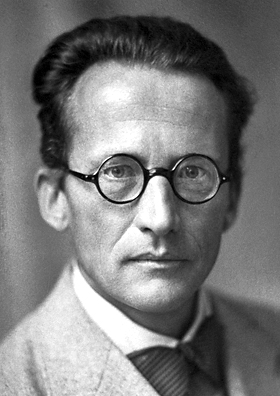
\includegraphics[width=\linewidth]{images/book4/schrodinger-1933.jpg}\par
{\footnotesize شرودنغر سنة 1933.}
\end{minipage}
\end{history}

\section{تمارين}

\begin{exercise}[$\star$]\label{exo:b3:quantum-model-systems:1}
إلكترون محصور في صندوق طوله (أ) \qty{1.00}{nm}، (ب)
\qty{0.50}{nm}. احسب $E_1$ بالجول وبالإلكترون فولت، وطول موجة
الانتقال $n = 1 \to 2$.
\end{exercise}

\begin{exercise}[$\star$]\label{exo:b3:quantum-model-systems:2}
اكتب المستويات الخمسة الأدنى \omterm{def:b3:quantum-model-systems:box}{لجسيم في صندوق} مكعب، بوحدة
$h^2/8mL^2$، مع \omterm{def:b3:quantum-model-systems:degenerate}{درجات انحلالها}.
\end{exercise}

\begin{exercise}[$\star$]\label{exo:b3:quantum-model-systems:3}
احسب \omterm{def:b3:quantum-model-systems:commutator}{المبدِّلين} $[\hat x^2,\hat p]$ و$[\hat p^2,\hat x]$ بتطبيقهما
على دالة $f(x)$.
\end{exercise}

\begin{exercise}[$\star$]\label{exo:b3:quantum-model-systems:4}
% ledger: diat:HCl.Be
علمًا أن $B = \qty{10.593}{cm^{-1}}$ للجزيء \ce{H^{35}Cl}، أعطِ طاقات المستويات $J = 0$ إلى 3 (بوحدة
\unit{cm^{-1}}) \omterm{def:b3:quantum-model-systems:degenerate}{ودرجات انحلالها}، وعزم
عطالة الجزيء.
\end{exercise}

\begin{exercise}[$\star\star$]\label{exo:b3:quantum-model-systems:5}
من أجل الحالة $\psi_n$ \omterm{def:b3:quantum-model-systems:box}{لجسيم في صندوق}، احسب $\langle x\rangle$ 
و$\langle x^2\rangle$. واحسب $\langle x^2\rangle$ من أجل $n = 1$ وقارنها
بالقيمة الكلاسيكية $L^2/3$ لجسيم يتساوى احتمال وجوده في أي موضع.
\end{exercise}

\begin{exercise}[$\star\star$]\label{exo:b3:quantum-model-systems:6}
% ledger: diat:H2.we, diat:D2.we
احسب طاقتي النقطة الصفرية التوافقيتين للجزيئين \ce{H2} و\ce{D2} بوحدة
\unit{kJ/mol} انطلاقًا من $\tilde\omega_e = \qty{4401.2}{cm^{-1}}$ 
و\qty{3115.5}{cm^{-1}}، والفرق بينهما. ما النسبة بين العددين الموجيين التي
تتوقعها من الكتلتين المختزلتين، وما مدى قرب النسبة المقيسة منها؟
\end{exercise}

\begin{exercise}[$\star\star$]\label{exo:b3:quantum-model-systems:7}
الدالة $\phi = Nx(L - x)$ تخمين تقريبي للحالة الأساسية في
الصندوق. نظّمها، ثم احسب تداخلها $\langle\psi_1|\phi\rangle$ مع
الحالة الأساسية الحقيقية.
\end{exercise}

\begin{exercise}[$\star\star$]\label{exo:b3:quantum-model-systems:8}
بيّن أن $\hat p = -\iu\hbar\,\dd/\dd x$ هرميتي من أجل الدوال التي
تنعدم عند طرفي فترة، وأن $\hat x\hat p$ ليس كذلك.
\end{exercise}

\begin{exercise}[$\star\star$]\label{exo:b3:quantum-model-systems:9}
نمذج الهكسا-1،3،5-ترايين بستة إلكترونات $\pi$ في صندوق طوله $6l$، حيث $l =
\qty{139.7}{pm}$ (خمس روابط ونصف رابطة عند كل طرف). تنبأ
بطول موجة امتصاصه الأول. هل الجزيء ملوَّن؟
\end{exercise}

\begin{exercise}[$\star\star\star$]\label{exo:b3:quantum-model-systems:10}
من أجل الحاجز النموذجي في الشكل ($V_0 = \qty{0.40}{eV}$، $a = \qty{50}{pm}$)
عند $E = V_0/2$، احسب $\kappa$ للبروتون وللديوترون، ثم النسبة $T_H/T_D$
بعلاقة الحاجز السميك. قارنها بالنسبة الدقيقة، 58.
\end{exercise}

\begin{exercise}[$\star\star\star$]\label{exo:b3:quantum-model-systems:11}
عامل إلكترونات $\pi$ الستة في البنزين كجسيمات على حلقة نصف قطرها
\qty{139.7}{pm} (المسافة C--C تساوي نصف قطر المسدس المنتظم).
املأ المستويات، ثم احسب طول موجة الانتقال من
أعلى مستوى مملوء إلى أدنى مستوى فارغ.
\end{exercise}

\begin{exercise}[$\star\star\star$]\label{exo:b3:quantum-model-systems:12}
من أجل الحالة $1s$ للهيدروجين، $\psi = (\pi a^3)^{-1/2}\eu^{-r/a}$. احسب
القيمتين المتوقعتين $\langle r\rangle$ و$\langle V\rangle$، وتحقق من أن
$\langle V\rangle = 2E_1$. (استعمل $\int_0^\infty r^n\eu^{-\beta r}\dd r =
n!/\beta^{n+1}$.)
\end{exercise}

\section{مسألة: كم طول الصبغة؟}

\begin{problem}[{مسألة نهاية الأسبوع --- نموذج الإلكترون الحر لثلاث
صبغات سيانينية: لماذا تخفق السلسلة العارية، وأي الانتقالات مسموح، وسلالم
الطاقة في الجزيء، وطول الصندوق الذي يوافق القياس}]
\label{pb:b3:quantum-model-systems:1}
% ledger: uvvis:cyanine, uvvis:carbocyanine, uvvis:dicarbocyanine, geo:C6H6.rCC, diat:HCl.we, diat:HCl.Be
تمتص ثلاث صبغات سيانينية متناظرة عند 524 و603 و711 نانومترًا في الإيثانول؛ 
وسلاسلها المترافقة، بين ذرتي النيتروجين وبإدخالهما، تضم $j = 5$ و7
و9 ذرات. خذ كل رابطة مساوية للطول $l = \qty{139.7}{pm}$، و$m_e =
\qty{9.109e-31}{kg}$، و$h = \qty{6.626e-34}{J.s}$، و$c = \qty{2.998e8}{m/s}$،
و$k = \qty{1.381e-23}{J/K}$، و$\qty{1}{eV} = \qty{1.602e-19}{J}$.

\medskip\noindent\textbf{الجزء الأول --- سلسلة عارية.}
\begin{enumerate}
  \item علّل لماذا تحمل السلسلة ذات $j$ ذرة $N = j + 1$ إلكترونًا $\pi$، 
        وأعطِ $N$ لكل صبغة.
  \item ما مستويات الصندوق التي هي أعلى مستوى مملوء وأدنى مستوى فارغ
        في الصبغة الأولى؟
  \item بيّن أن الامتصاص الأول يقع عند $\lambda = 8mcL^2/h(N+1)$.
  \item أعطِ الطول العاري $L_0 = (j - 1)l$ لكل سلسلة.
  \item احسب $\lambda$ لكل صبغة مع $L = L_0$.
  \item قارن بالقيم المقيسة. في أي اتجاه يخطئ النموذج،
        وماذا يقول ذلك عن $L$؟
\end{enumerate}

\medskip\noindent\textbf{الجزء الثاني --- أي الانتقالات مسموح.}
شدة الانتقال $n \to n'$ متناسبة مع $|\langle
\psi_n|x - L/2|\psi_{n'}\rangle|^2$.
\begin{enumerate}[resume]
  \item بيّن أن $\psi_n$ متناظرة بالنسبة إلى مركز الصندوق من أجل $n$ فردي
        وضد متناظرة من أجل $n$ زوجي.
  \item استنتج أن التكامل ينعدم حين يكون $n + n'$ زوجيًا.
  \item هل الانتقال HOMO $\to$ LUMO مسموح في كل صبغة؟
  \item في الصبغة الثانية، هل الانتقال من HOMO إلى المستوى
        الذي يعلو LUMO مسموح؟ ومن المستوى الذي تحت HOMO إلى LUMO؟
  \item في النموذج، عند أي طول موجة (كجزء من طول الموجة الأول)
        يقع الانتقال المسموح التالي انطلاقًا من HOMO؟
  \item لماذا تصمد قاعدة كهذه، مستنتجة من التناظر وحده، أمام
        فجاجة النموذج؟
\end{enumerate}

\medskip\noindent\textbf{الجزء الثالث --- سلالم الطاقة في الجزيء.}
\begin{enumerate}[resume]
  \item حوّل امتصاص الصبغة الثانية إلى طاقة بالإلكترون فولت.
  \item لاهتزاز \ce{HCl} العدد الموجي $\tilde\omega_e = \qty{2991}{cm^{-1}}$:
        حوّل كمّه إلى الإلكترون فولت.
  \item لدوران \ce{HCl} الثابت $B = \qty{10.59}{cm^{-1}}$: حوّل
        الفجوة بين $J = 0$ و$J = 1$ إلى الميلي إلكترون فولت.
  \item احسب $kT$ بالميلي إلكترون فولت عند \qty{298}{K}.
  \item أي أنواع الإثارة مأهولة في درجة حرارة الغرفة؟
  \item في أي مناطق الطيف تُرصد الانتقالات الإلكترونية والاهتزازية
        والدورانية؟
\end{enumerate}

\medskip\noindent\textbf{الجزء الرابع --- الصندوق الموافق.}
\begin{enumerate}[resume]
  \item انطلاقًا من القيمة المقيسة 603 نانومترًا، احسب الطول $L$ الذي يجب أن يكون
        لصندوق الصبغة الثانية.
  \item بكتابة $L = L_0 + 2\delta$، استنتج $\delta$.
  \item بهذه القيمة للمقدار $\delta$، تنبأ بقيمة $\lambda$ للصبغة الأولى؛ وأعطِ
        الخطأ النسبي.
  \item السؤال نفسه للصبغة الثالثة.
  \item فسّر $\delta$: إلى أين تمتد إلكترونات $\pi$ بعد
        ذرتي النيتروجين؟
  \item عبّر عن $\delta$ بأطوال الروابط، واذكر نتيجة
        المسألة: الامتداد الفعلي للصندوق عند كل طرف.
\end{enumerate}
\end{problem}
